%%%%%%%%%%%%%%%%%%%%%%% Boundary-Layer Meteorology 2019 Template %%%%%%%%%%%%%%%%%%%%%%%%%


% \begin{filecontents*}{example.eps}
% gsave
% newpath
%   20 20 moveto
%   20 220 lineto
%   220 220 lineto
%   220 20 lineto
% closepath
% 2 setlinewidth
% gsave
%   .4 setgray fill
% grestore
% stroke
% grestore
% \end{filecontents*}

\RequirePackage{fix-cm}
\documentclass[smallextended]{svjour3}
\smartqed
\usepackage{appendix}
\usepackage{amsmath,amssymb}
\usepackage{graphicx}
\usepackage{lineno}
\usepackage{array}
\usepackage{longtable}
\usepackage{natbib}
\setcitestyle{aysep={}}
\linenumbers

\newcommand*\patchAmsMathEnvironmentForLineno[1]{%
\expandafter\let\csname old#1\expandafter\endcsname\csname #1\endcsname
\expandafter\let\csname oldend#1\expandafter\endcsname\csname end#1\endcsname
\renewenvironment{#1}%
{\linenomath\csname old#1\endcsname}%
{\csname oldend#1\endcsname\endlinenomath}}%
\newcommand*\patchBothAmsMathEnvironmentsForLineno[1]{%
\patchAmsMathEnvironmentForLineno{#1}%
\patchAmsMathEnvironmentForLineno{#1*}}%
\AtBeginDocument{%
\patchBothAmsMathEnvironmentsForLineno{equation}%
\patchBothAmsMathEnvironmentsForLineno{align}%
\patchBothAmsMathEnvironmentsForLineno{flalign}%
\patchBothAmsMathEnvironmentsForLineno{alignat}%
\patchBothAmsMathEnvironmentsForLineno{gather}%
\patchBothAmsMathEnvironmentsForLineno{multline}%
}

\usepackage[dvipsnames]{xcolor}
\newcommand{\cg}{\textcolor{WildStrawberry}}


\begin{document}

\title{Significant wind disturbances induced by giant dunes.}

\author{Cyril Gadal \and Pauline Delorme \and Clément Narteau \and
        Giles Wiggs \and Matthew Baddock \and Joanna M. Nield \and Philippe Claudin }

\institute{C. Gadal \at
              Institut de Mécanique des Fluides de Toulouse (IMFT), Université de Toulouse, CNRS, INPT, UPS, Toulouse, France \\
              \email{cyril.gadal@imft.fr}
           \and
           S. Author \at
              second address
            \and
            T. Author \at
            third address
}

\date{Received: DD Month YEAR / Accepted: DD Month YEAR}

\maketitle

\begin{abstract}
  abstract
\keywords{Boundary layer \and Turbulent flow \and Sand dunes \and Fluide-structures interactions}
\end{abstract}

\newpage

\section{Introduction}

Whenever a flow encounters an obstacle, various types of interactions can arise depending the different time and lengths scales involved. In the case of atmospheric flows, this depends mainly on the part of the vertical structure of the atmosphere, schematically composed of a turbulent boundary layer topped by a turbulence-free part, with which the obstacle interacts \citep{Stull1988}.
%
At the largest scale, the feedback of mountains on the stratified flow of the free atmosphere results in wave generation as well as significant wind disturbances, such as foehn winds in the lee side \citep{refs}. Inside the boundary layer, the interaction between a turbulent flow and hilly surfaces is for example key to the understanding ocean surface wind-driven waves, or eolian bedforms in desert \citep{Belcher1998, Sullivan2010, Courrech2015}.

Indeed, eolian sand dunes typically emerge from the feedback of the topography on the turbulent flow, which speeds up close to the dune crest \citep{Rubin1987, Charru2013, Courrech2014}. Later on, when the dune reaches an intermediate size, it may also induce significant wind deflections. This can impact the sediment pathways of coastal systems \citep{Hesp2015}, or affect the collective behavior of dune populations with long-range interactions due to flow disturbances induced by each individual \citep{Smith2017, Bacik2020}. As the dunes increase in size by collisions and coarsening, they sometimes reach a giant size, comparable to the boundary layer depth, thus inducing interactions not only with the turbulent flow of the ABL, but also with the free atmosphere~\citep{andreotti2009}. However, the wind disturbances induced by these giant dunes have never been quantified.

The study of the impact of obstacles on the atmospheric flows allow its incorporation within meteorological numerical model. Therefore, they mainly become limited by the precision of the included topographical data, as well as the spatial grid of the model. For example, the latest climate reanalysis, ERA5-Land, is limited by its $9~\textup{km}$ spatial resolution, while including the data $30$-m Digital Elevation Models (DEMs) of the shuttle radar topography mission \citep{Farr2007, munoz2021}. As such, it can not reproduce the flow disturbances induced by giant dunes, which have a typical length scale $\sim 1~\textup{km}$.

Here, we compare the wind predictions from the ERA5-Land dataset to local measurements in four different places across the Namib desert. In places with no significant topographies smaller than the model grid, we show that both wind datasets agree with each other. On the contrary, in places with giant dunes, we show that they may differ for some specific meteorological conditions, that we link to the circadian cycle of the ABL. We thus highlight the importance of the mid-scale topographies for local wind regimes, and its implications in the case of sand seas for smaller-scale eolian bedforms.


\section{Wind regimes across the Namib Sand Sea}

In this study, we focus on four places across and nearby the Namib desert, highlighting different environments (see Fig.~\ref{Fig1}).
%
The Adamax station is located near the Adamax salt pan, in a highly vegetated area. The Huab station, located on the coast at the outlet of the Huab river is an arid environment exhibiting $60$-m scale barchan dunes. While these two stations are in environments with no mid-scale topography, this is not the case for the Deep Sea and South Namib stations. Both are located in the interdune between giant linear dunes with kilometric wavelengths and superimposed patterns. In this section, we describe and compare the wind regimes resulting from the available datasets in each station.

  \begin{figure}
    \centering
    \includegraphics[scale=1]{Figures/Figure1.pdf}
    \caption{Wind data used in this study \textbf{a}: Location of the studied sites. \textbf{b--e}: Satellite images of the studied sites (Google-Earth, Maxar Technologies, CNES/Airbus). In each subplot, the left and right wind roses represent the data from the ERA5Land climate reanalysis and the in situ stations, respectively. Note that the bars show the direction towards which the wind blows. The red dots show the location of the in situ stations.}
    \label{Fig1}
  \end{figure}

  \subsection{Datasets}

  Two wind datasets are used in this study. First, local winds are provided by stations situated in the four different places (see Fig.~\ref{Fig1}). The wind strength and direction are measured every 10 minutes by cup anemometers and wind vanes, at heights between $2$~m and $3$~m depending on the station. The available period of measurements ranges from 1 to 5 discontinuous years distributed between 2012 and 2020 (see Fig.~\ref{Fig1_supp}). We checked that at least one complete seasonal cycle is available at each station.
  %
  Then, regional winds are extracted at the same locations and periods from the ERA5-Land dataset, which is a replay at a smaller spatial resolution of ERA5, the latest climate reanalysis from the ECMWWF \citep{Hersbach2020, munoz2021}. It provides hourly estimates of the 10-m wind velocity and direction at a spatial resolution of $\sim 9~\textup{km}$ ($0.1^\circ\times0.1^\circ$).

  For comparison, the local measurements are averaged into 1-hr bins centered on the temporal scale of the ERA5-Land estimates (see Fig.~\ref{Fig2_supp}). As the wind velocities of both datasets are provided at different heights, we convert them into shear velocities (see SI section 1), characteristic of the whole turbulent wind profile within the atmospheric boundary layer, which are then used together with the wind direction for further analysis. The resulting wind data are shown on the wind roses of Fig.~\ref{Fig1}(b--e).

  Finally, the dune properties are computed using autocorrelation on the 30-m Digital Elevation Models (DEMs) of the shuttle radar topography mission \citep{Farr2007}. For the South Namib and Deep Sea stations, we obtain respectively orientations of $85^\circ$ and $125^\circ$, wavelengths of $2.6~\textup{km}$ and $2.3~\textup{km}$ and amplitudes of $45~\textup{m}$ and $20~\textup{m}$ (see Fig.~\ref{Fig4_supp} for more details).

  \subsection{Agreement between local and regional winds}

  \begin{figure}
    \centering
    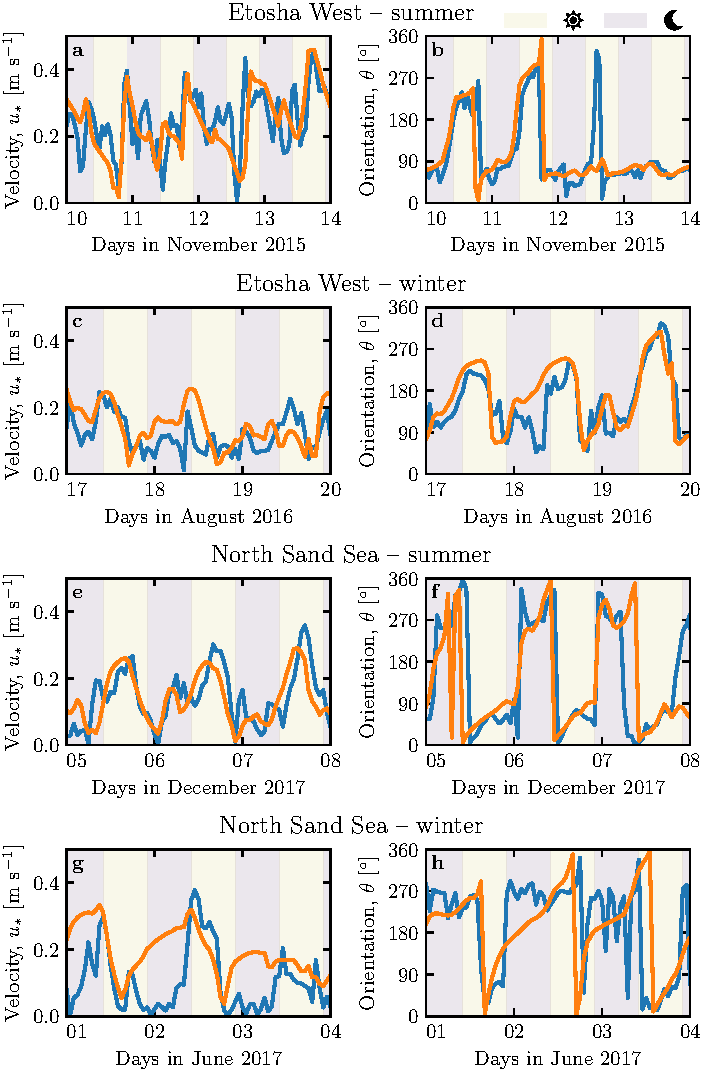
\includegraphics[scale=1]{Figures/Figure2.pdf}
    \caption{Temporal comparison between the wind data coming from the Era5Land climate reanalysis (orange lines) and from the in situ measurements (blue lines). \textbf{a--b}: Huab station. \textbf{c--d}: Deep Sea station in winter. \textbf{e--f}: Deep Sea station in summer.}
    \label{Fig2}
  \end{figure}

  The obtained wind regimes are shown in figure~\ref{Fig1}. In the Namib, the regional wind patterns are essentially controlled by the see breeze, resulting in strong northward components (sometimes slightly deviated by the large scale topography) present in all regional wind roses \citep{lancaster1985}. These daily winds are dominant during the second-half of the year (Septembre-January). In winter, an additional easterly component can be recorded during the night, induced by the combination of katabatic winds forming on the mountains, and infrequent `berg' winds, which are responsible of the high wind velocities observed \citep{lancaster1984}. The frequency of these easterly components decreases from the inland to the coast, resulting in bidirectional wind regimes within the Namib Sand Sea and at the Adamax salt pan (Fig.~\ref{Fig1}b, \ref{Fig1}d and \ref{Fig1}e) and a unidirectional wind regime on the coast at the outlet of the Huab River (Fig.~\ref{Fig1}c).

  In the case of the Adamax and Huab stations, the regional wind roses qualitatively match those corresponding to the local in situ measurements. However, for the Deep Sea and South Namib stations, the local wind roses exhibit additional components aligned with the giant dune orientation visible on the satellite images (Fig.~\ref{Fig1}c--d).
  %
  Indeed, the analysis of the wind speed and direction time series shows that the agreement between the local and regional datasets is always verified when no mid-scale topography are present (Fig.~\ref{Fig2}a--b) and Fig.~\ref{Fig5_supp}). In contrast, for the stations within the giant dune field, we observe that this agreement is limited to the Septembre--January time periods (Fig.~\ref{Fig2}c--d).

  \subsection{Influence of the giant dunes on local wind regimes}
  \label{section_data_feedback}

  When giant dunes are present, in the February--August period, the local and regional winds match only during the morning, i.e when the southerly/southwesterly sea breeze dominates (see Fig.~\ref{Fig2}(e--f), Fig.~\ref{Fig3} and Fig.~\ref{Fig6_supp}). In the late afternoon and during the night, when the northwesterly `berg' and katabatic winds blow, the two datasets differ. In this case, the angular wind distribution of the local measurements exhibits two additional modes separated of $\simeq 180^\circ$, each corresponding to the giant dune alignement (purple frame in Fig.~\ref{Fig3} and Fig.~\ref{Fig6_supp}, as well as Fig.~\ref{Fig7_supp}). This deviation is also associated with a global attenuation of the wind strength (Fig.~\ref{Fig8_supp}). Remarkably, all these figures show that this process occurs for low wind velocities, typically for $u_{*} < 0.1~\textrm{m}~\textrm{s}^{-1}$. For shear velocities larger than $0.25~\textrm{m}~\textrm{s}^{-1}$, this wind reorientation does not occur. Finally, for intermediate shear velocities, both reorientation along the dune crest and no reorientation are observed (Fig.~\ref{Fig7_supp}).


  \begin{figure}
    \centering
    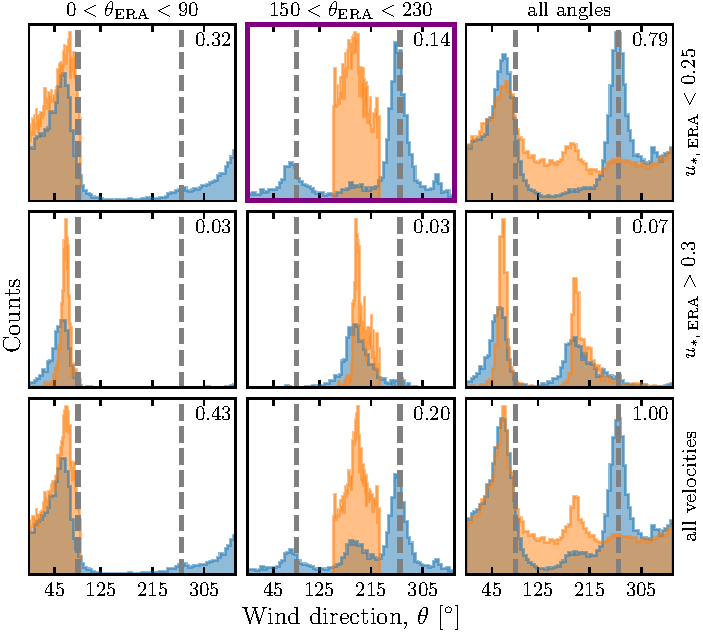
\includegraphics[scale=1]{Figures/Figure3.pdf}
    \caption{Distributions of wind direction at the Deep Sea Station for the Era5Land climate reanalysis (orange) and the in situ measurements (blue). In each subplot, both distributions are plotted from the same time steps, selected with constraints on the wind direction (columns) and/or wind velocity (rows) in the Era5Land dataset. The vertical gray dashed lines indicate the dune orientation, and the top right numbers the percentage of the total number of time steps selected in each subplot. The purple frame highlights the regime (small wind velocities, nocturnal summer wind) during which the wind data from both datasets differs. A similar figure can be obtained for the Deep Sea station (see Fig.~\ref{Fig6_supp}).}
    \label{Fig3}
  \end{figure}


  \section{Influence of the circadian cycle of the atmospheric boundary layer}

  In the case of linear ridges, dune-induced flow disturbances have mainly been related to the incident wind direction~\citep{Walker2009, Hesp2015}. In our case, it is unlikely to be the dominant parameter, as the most deflected wind for both stations is the most perpendicular, where it should be winds with incident directions between $30^{\circ}$ and $70^{\circ}$~\citep{Hesp2015}. An important observation is the difference in behavior between low and high wind velocities, which suggests a change in the hydrodynamical regime.

  Previous studies have linked atmospheric flow around and over topographical obstacles to the vertical structure of the atmosphere \citep{Stull1988}. More particularly, dunes evolves in its lower part, the turbulent atmospheric boundary layer (ABL), typically characterized by a logarithmic wind profile and a vertically constant potential temperature. Above, the free atmosphere (FA) is a stably stratified zone in which turbulence is negligible, and where the flow is usually considered as incompressible and inviscid. In the middle, a transitional layer, also known as entrainment zone, is characterized by a sharp increase of the potential temperature, which traps the turbulence resulting from the surface friction below it.

  In the following, we sum-up the dominant numbers leading to different hydrodynamical interactions with topographical obstacles, and interpret the data with respect to the corresponding physical mechanisms.

  \begin{figure}
    \centering
    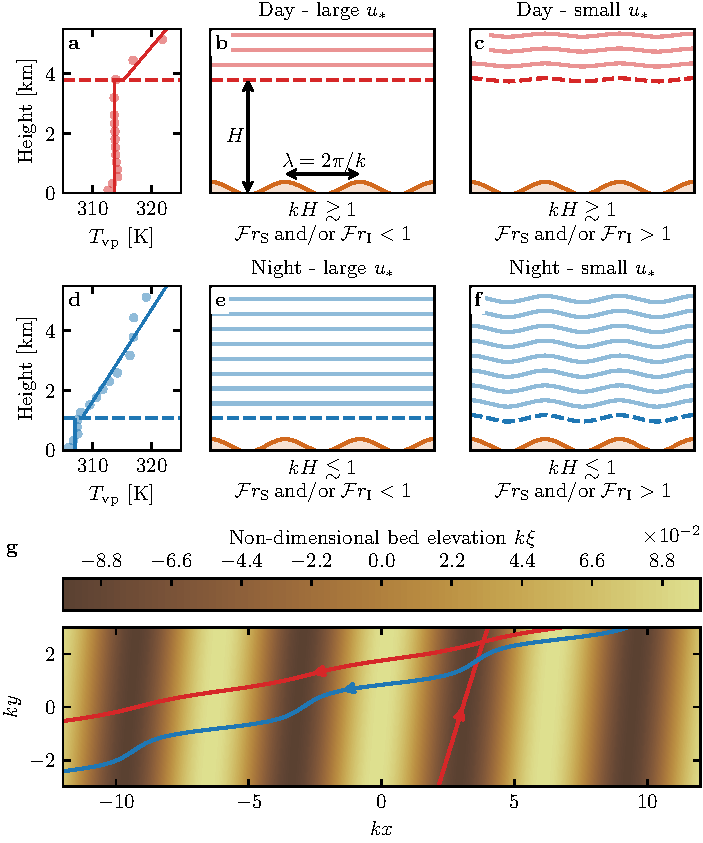
\includegraphics[scale=1]{Figures/Figure4.pdf}
    \caption{\textbf{a}: Vertical profiles of the virtual potential temperature at 2 different time steps (blue - 29/11/2012 - 1100 UTC, red - 21/03/2017 - 1200 UTC) at the Deep Sea station. Dots: data from the ERA5 reanalysis. Transparent dashed lines: boundary layer height given by the ERA5 reanalysis, calculated from the bulk Richardson number \citep{seidel2012}. Plain lines: vertical (boundary layer) and linear (free atmosphere) fits to estimate the stratification properties. \textbf{b--d}: Sketches representing the interaction between the giant dunes and the atmospheric flow for different meteorological conditions. \textbf{e}: Streamlines qualitatively representing the effect of flow confinement, in the case of the Deep Sea station. The red and straight blue lines are calculated from the unconfined case, representing the situations \textbf{b--c}. The sinuous blue line represents the confined case of \textbf{d}. For details on their derivation, see Appendix.}
    %
    %
    % calculated from equation~\eqref{Tau}. Note that topography and wind geometry represent the case of the Deep Sea station. For the red and straight blue lines, $(\mathcal{A}_{0}, \mathcal{B}_{0}) = (3.8, 1.3)$, calculated from the unbounded case of \citep{Fourriere2010}, and representing the situations \textbf{b--c}. For the sinuous blue line, $(\mathcal{A}_{0}, \mathcal{B}_{0}) = (8, 2)$, representing the confined case of \textbf{d}.}
    \label{Fig4}
  \end{figure}

  \subsection{Relevant non-dimensional parameters and physical modeling}
  \label{theoretical_framework}

  Flow deflection over ridges can be simplistically understood from a balance between inertia and pressure gradients~\citep{Hesp2015}. As the flow approaches the ridge crest, the compression of the streamlines results in larger flow velocities, and thus lower pressures~\citep{Rubin1987}. An incident flow oblique to the ridge is then deflected towards lower pressure zones, i.e towards the crest. Turbulent dissipation at the bottom and non-linearities tends to increase this effect downstream, resulting in along the crest wind deflection in the lee side~\citep{Hesp2015, Gadal2019}.

  Another way to increase the flow deflection is its confinement below a capping surface, that result in further streamline compression. This happens when the flow disturbance induced by the obstacle reaches the surface. As obstacles typically disturb flow over a characteristic height similar to their width, this is well captured by the parameter $k H$, where $k = 2\pi/\lambda$ is the wavenumber and $H$ the ABL depth. Here, the giant dunes have kilometric wavelengths, such that $0.02 \lesssim k H \lesssim 5$, and they interact most of the time with the capping layer and the stratified free atmosphere above \citep{andreotti2009}.

  Note that the ability of the capping layer and stratification to accommodate a perturbation induced by the topography directly impacts the strength of this confinement effect (Fig.~\ref{Fig4}). This is typically quantified using surface and internal Froude numbers
  \citep{Vosper2004, Stull2006, Sheridan2006, Hunt2006, Jiang2014}:
  \begin{equation}
        \mathcal{F}r_{\textup{S}} = \displaystyle\frac{U}{\sqrt{\displaystyle\frac{\Delta\rho}{\rho}gH}}, \, \mathcal{F}r_{\textup{I}} = \displaystyle\frac{k U}{N},
  \end{equation}
  where $U$ is the wind velocity at the top of the ABL, $\rho$ its average density, $\Delta\rho$ the density jump between the ABL and the FA and $N$ is the Brunt-Väisälä frequency, characteristic of the stratification.

  The smallest wind disturbances are expected during the day, when the ABL depth is comparable to the dune wavelength ($k H \gtrsim 1$) and for large wind velocities, which correspond to a weak confinement situation (Fig.~\ref{Fig4b}). On the contrary, large wind disturbances are expected to occur during the night, when the confinement is mainly induced by shallow ABL (Fig.~\ref{Fig4d--f}). Note that this strong confinement can be somewhat reduced in the case of strong winds (corresponding to large Froude numbers, see Fig.~\ref{Fig4f}), explaining the threshold in velocity observed in the data (see section~\ref{section_data_feedback}).

  \subsection{Flow regime diagrams}

  In the spirit of \citet{Sheridan2006}, we aim to compute flow regime diagrams in the space defined by the three relevant non-dimensional numbers presented above, $\left(k H,\, \mathcal{F}r_{\textup{S}}, \, \mathcal{F}r_{\textup{I}}\right)$. They are calculated from the time series of the geopotential, temperature and specific humidity vertical profiles available in the ERA5 climate reanalysis (see SI~\ref{?}). The relative velocity modulation is computed as
  %
  \begin{equation}
    \delta_{\textup{u}} = \frac{u_{*}^{\textup{ERA}} -  u_{*}^{\textup{station}}}{u_{*}^{\textup{ERA}}},
  \end{equation}
  %
  and the flow deviation as the minimal angle between the wind orientation in the two datasets:
  %
  \begin{equation}
    \delta_{\theta} = \left\vert \textup{min}\left(\left[\theta_{\textup{ERA}} - \theta_{\textup{station}}\right] \, \textup{mod.} \, 360, \left[\theta_{\textup{station}} - \theta_{\textup{ERA}}\right] \, \textup{mod.} \, 360\right) \right\vert,
  \end{equation}
  %

  When these two variables are represented in the marginal spaces $(k H,\, \mathcal{F}r_{\textup{S}})$ and $(k H,\, \mathcal{F}r_{\textup{I}})$, different regime emerges (Fig.~\ref{Fig5}). The small wind disturbances ($\delta_{\theta} \to 0$, $\delta_{\textup{u}} \to 0$) are located in the top-right part of the diagrams, corresponding to a regime mixing low-interactions ($k H$ large enough, Fig.~\ref{Fig4}b) and low-confinement ($\mathcal{F}r_{\textup{S}}, \, \mathcal{F}r_{\textup{I}}$ large enough, Fig.~\ref{Fig4}c).

  Lower values of $k H$ (stronger interaction) or Froude numbers (stronger confinement) then both leads to an increase in wind disturbances, both in terms of orientation and velocity. Interestingly, the limit of no-interactions between the topography and the boundary layer structure ($k H \gg 1$), in which the properties of the capping layer and the stratification become irrelevant (Fig.~\ref{Fig4}b--\ref{Fig4}c), is never reached here, in the case of giant dunes.
  %
  Below a threshold value of $k H \simeq 0.3$, wind disturbance occurs independently of the Froude numbers value. However, the latter seem to control a transition between from damped to amplified wind velocities within the interdune (Fig.~\ref{Fig5}c--\ref{Fig5}d), for which we do not have an explanation.


  \begin{figure}
    \centering
    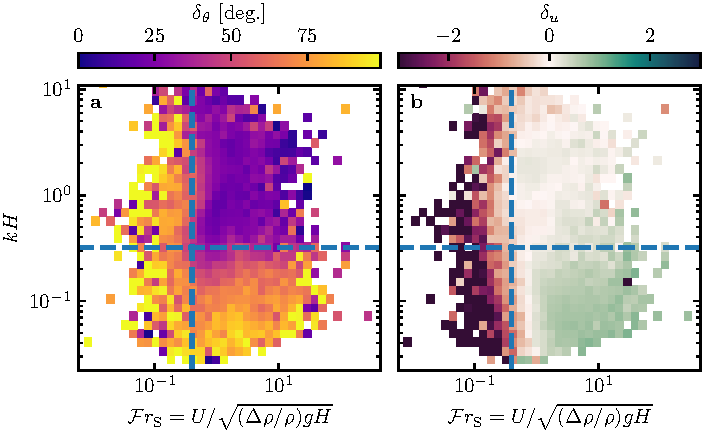
\includegraphics[scale=1]{Figures/Figure5.pdf}
    \caption{Regime diagrams of the wind deviation $\delta_{\theta}$ and relative attenuation/amplification $\delta_{u}$ in the space $(\mathcal{F}r_{\textup{S}}, \, kH)$, containing the data from both the Deep Sea and South Namib stations. Blue dashed lines empirically delimit the different regimes. The point density in each bin of the diagrams is shown in Fig.~\ref{Fig11_supp}. The regime diagrams in the spaces $(\mathcal{F}r_{\textup{I}}, \, kH)$ and $(\mathcal{F}r_{\textup{I}}, \, \mathcal{F}r_{\textup{S}})$ are shown in Fig.~\ref{Fig12_supp}.}
    \label{Fig5}
  \end{figure}

\section{Discussion}

 The comparison of local and regional wind data gives a direct evidence of the giant dunes feedback on the flow. In flat areas, the matching between both datasets highlights the ability of the latest generation of climate reanalysis to predict the wind flow up to scales $\sim 10~\textrm{km}$, i.e the grid model. When smaller scale topographies are present (giant dunes in our case), locally measured wind regimes may significantly differ from the regional ones. Furthermore, we link these disturbances induced by the dunes to their interaction with the lower part of the atmospheric vertical structure, and more specifically to its circadian variability. During the day, the top of the ABL is high enough to limit the interaction of the capping layer and the FA stratification with the giant dunes, resulting in a low flow confinement, and thus small wind disturbances. During the night, the small ABL height induces a stronger flow confinement, associated with large wind deviation and acceleration or deceleration. Interestingly, we also found that this effect could be counterbalanced by the presence of large wind velocities, capable of deforming the capping layer and/or the FA stratification and thus decreasing the confinement effect.

 Simple linear model such as the one of \citet{andreotti2009} also suggests that larger wind disturbances occur under strong flow confinement such as described above. However, they are unable to reproduce the magnitude of the observed deviations, probably due to the presence of hydrodynamical non-linear effects, negligible in low confinement situations, but not otherwise (see Fig.~\ref{Fig12_supp} and Appendix 1). Another limit in the comparison between theoretical predictions and measured is induces by the the single-point measurements. To have reliable representations of the flow structures related to wind disturbances, additional measurements in different places on and near the same topographical obstacle are needed.

 This study highlights the interaction between giant dunes and the atmospheric boundary layer, thus supporting for example the way the capping layer acts as a bounding surface limiting dune growth \citep{andreotti2009, gunn2021}. This interaction also have implications at smaller scales, where bedforms then develop from the disturbed wind instead of the regional one. Differences between larger and smaller scale (thus older and more recent) dune patterns are observed ubiquitously, and have sometimes in the literature been attributed to climatic changes in wind regimes \citep{refs}. Here, we suggest using this feedback mechanism that current winds can explain dune patterns at all scales, such as the linear dunes ($\sim 50$ m -wide) elongating within the interdune between two giant linear dunes ($\sim 2$ km -wide) in the Namib Sand Sea (see Fig.~\ref{Fig6}).


\begin{figure}
  \centering
  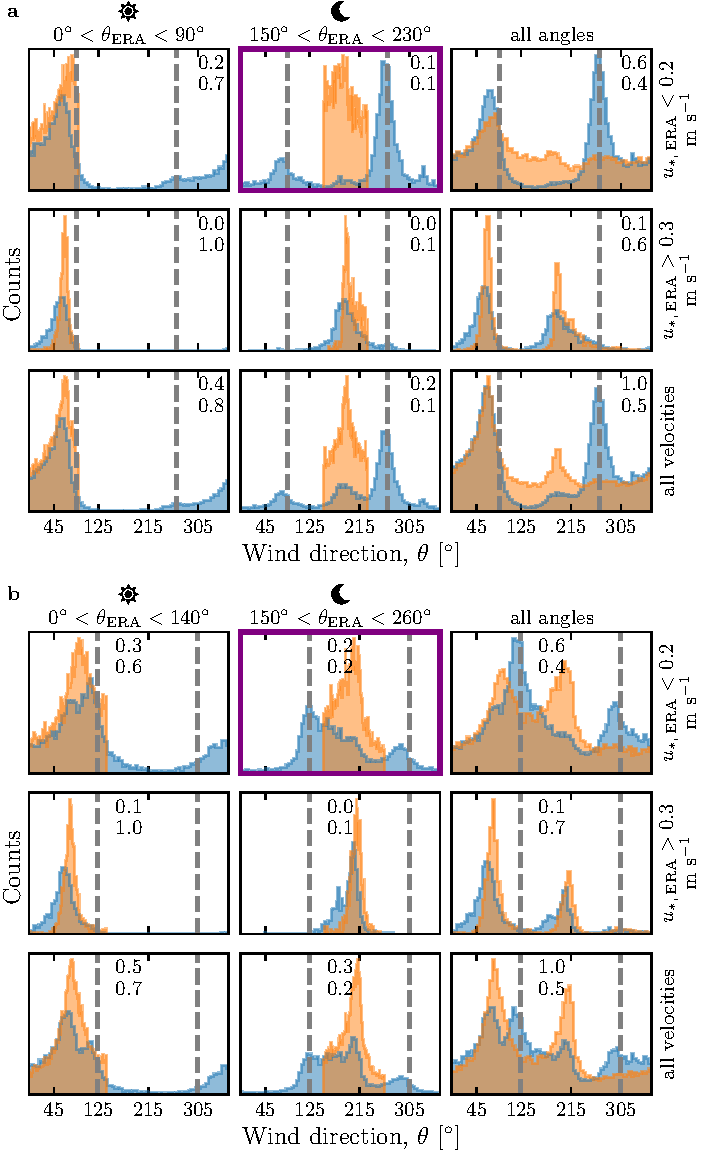
\includegraphics[scale=1]{Figures/Figure6.pdf}
  \caption{Implications for smaller scale patterns in (a) the South Namib and (b) Deep Sea. The ellipses indicates the different types of elongating dunes, at large (plain) and small scale (dashed). The dune orientations are calculated using the model of \citet{Cour14} from the sand flux angular distributions, shown here for typical sand quartz grains of $180~\mu$m. The double blue and single red arrows correspond to the two possible dune growth mechanisms, bed instability and elongation, respectively. Likewise, plain arrows are calculated from the ERA5-Land datasets, and dashed arrows from the in situ measurements. Wedges show the uncertainty on the orientation calculation, and the arrows correspond to typical parameters found in the literature, i.e a grain diameter of $180~\mu$m and a flux-up ratio of 1.6. The green dots indicate the position of the measurement stations. See Appendix 2 for details.}
  \label{Fig6}
\end{figure}

\begin{acknowledgements}
These should follow the concluding section of the paper and precede the References and any appendices, if they are present. The acknowledgements section does not require a section number.
\end{acknowledgements}

\section*{Appendix 1: ABL turbulent wind model}

Following the work of \citet{Fourriere2010} and \citet{Andreotti2012}, we briefly expose in this section the linear response of a turbulent flow to a small aspect ratio perturbation of the topography $\xi$. As this topography can be decomposed into several sinusoidal modes, we focus on the response to a sinusoidal topography as:
\begin{equation}
  \xi = \xi_{0}\cos\left[k\left(\cos(\alpha)x + \sin(\alpha)y\right)\right],
\end{equation}
which is also a good approximation to the giant dunes observed in the Deep Sea and South Namib Station (see Fig~\ref{Fig1} and Fig~\ref{Fig4_supp}). Here, $x$ and $y$ are the streamwise and spanwise coordinates, $k=2\pi/\lambda$ the wavenumber of the sinusoidal perturbation, and $\alpha$ its crest orientation, calculated with respect to the $y$--direction.

In terms of basal shear stress $\tau = \rho u_{*}^{2}$, the flow response can then generally be written in as:
\begin{align}
  \tau_{x} & = \tau_{0}\left(1 + k\xi_{0}\sqrt{\mathcal{A}_{x}^{2} + \mathcal{B}_{x}^{2}}\cos\left[k\left(\cos(\alpha)x + \sin(\alpha)y\right) + \phi_{x}\right]\right), \\
  \tau_{y} & = \tau_{0}k\xi_{0}\sqrt{\mathcal{A}_{y}^{2} + \mathcal{B}_{y}^{2}}\cos\left[k\left(\cos(\alpha)x + \sin(\alpha)y\right) + \phi_{y}\right],
\end{align}
where $\tau_{0}$ is the basal shear stress on a flat bed, and $\phi_{x, y} = \tan^{-1}\left(\mathcal{B}_{x, y}/\mathcal{A}_{x, y}\right)$. The in--phase and in--quadrature hydrodynamical coefficients $\mathcal{A}_{x, y}$ and $\mathcal{B}_{x, y}$ are functions of the flow conditions, i.e the bottom roughness, the free surface or the incident flow direction \citep{Fourriere2010, andreotti2009, Andreotti2012, Charru2013}.

\citet{Andreotti2012} have shown that the impact of the incident wind direction can be well approximated by the following expressions:
\begin{align}
  \mathcal{A}_{x} & = \mathcal{A}_{0}\cos^{2}\alpha, \\
  \mathcal{B}_{x} & = \mathcal{B}_{0}\cos^{2}\alpha, \\
  \mathcal{A}_{y} & = \displaystyle\frac{1}{2}\mathcal{A}_{0}\cos\alpha \sin\alpha, \\
  \mathcal{B}_{y} & = \displaystyle\frac{1}{2}\mathcal{B}_{0}\cos\alpha \sin\alpha,
\end{align}
where $\mathcal{A}_{0}$ and $\mathcal{B}_{0}$ are now two coefficients independent of the dune orientation $\alpha$. In the case of a fully turbulent boundary layer capped by a free atmosphere capping, they now only depend on $k H$, $k z_{0}$, $\mathcal{F}r_{\textup{I}}$ and $\mathcal{F}r_{\textup{S}}$, as detailed by \citet{andreotti2009}. More specifically, their variation in the marginal spaces $(k H,\, \mathcal{F}r_{\textup{S}})$ and $(k H,\, \mathcal{F}r_{\textup{I}})$ are shown in Fig.~\ref{Fig12_supp}.

Typical values for the unconfined case are therefore $\mathcal{A}_{0} = 3.4$ and $\mathcal{B}_{0} = 1$. In our case of giant dunes with $k\xi_{0} \sim 0.1$, significant wind disturbances are then expected when $\sqrt{\mathcal{A}_{0}^{2} + \mathcal{B}_{0}^{2}} \sim 10$. However, this is also the limit of the linear regime where this theoretical model is applicable, as hydrodynamical non-linearities become significant when $k\xi_{0}\sqrt{\mathcal{A}_{0}^{2} + \mathcal{B}_{0}^{2}} \sim 1$.

\section*{Appendix 2: Sediment transport and dune morphodynamics}

Here, we briefly detail the sediment transport and dune morphodynamics theoretical framework leading to the prediction of sand fluxes and dune orientations from wind data.

The sediment fluxes can been directly linked to the wind basal shear stress at each time steps $t$ from transport laws, whose exact forms depends on the sediment transport mechanisms taken into account. In this work, we following the recent work of \citet{Pahtz2020}, where the sediment flux $q_{\textup{sat}}$ on a flat bed made of loose sand can be expressed as:
\begin{equation}
  \label{transport_law}
  \frac{q_{\textup{sat, t}}}{Q} = \frac{2\sqrt{\Theta_{\textup{th}}}}{\kappa\mu}\left(\Theta_{t} - \Theta_{\textup{th}}\right)\left(1 +\frac{C_{\textup{M}}}{\mu}\left[\Theta_{t} - \Theta_{\textup{th}}\right]\right),
\end{equation}
where $\kappa = 0.4$ is the von Kármán constant, $C_{\rm M}=1.7$ a constant, $Q = d\sqrt{(\rho_{\textup{s}} - \rho)gd/\rho}$ is a characteristic flux, with $\rho_{\textup{s}} = 2.6~\textup{g}~\textup{cm}^{-3}$ and $d=180~\mu\textup{m}$ the grain density and diameter, and $g$ the gravitational acceleration. The friction coefficient $\mu$ is taken to be the avalanche slope of the granular material, i.e $\sim 0.6$. Finally, the Shields number is defined as $\Theta = \rho u_{*, t}^{2}/(\rho_{\textup{s}} - \rho)gd$, and its threshold value for incipient sediment transport as been calibrated using laboratory experiments to $\Theta_{\textup{th}} = 0.0035$.

The dune orientations are then predicted from the dimensional model of \citet{Courrech2014}. The orientation $\alpha$ corresponding the bed instability is then the one that maximizes the following growth rate:
\begin{equation}
  \sigma \propto \frac{1}{H W T}\int_{t}  q_{\textup{crest}, t}\vert \sin\left(\theta_{t} - \alpha\right) \vert,
\end{equation}
where $H$ and $W$ are dimensional constants representing the dune height and width, respectively. The flux at the crest is expressed as:
\begin{equation}
  q_{\textup{crest}, t} = q_{\textup{sat}, t}\left[1 + \gamma\vert\sin\left(\theta_{t} - \alpha\right)\vert\right],
\end{equation}
where the flux-up ratio $\gamma$ has been calibrated to 1.6 using field studies, underwater laboratory experiments and numerical simulations. Similarly, the dune orientation corresponding to the elongation mechanism is the one that verifies:
\begin{equation}
  \tan(\alpha) = \frac{\langle q_{\textup{crest}, t}(\alpha) \boldsymbol{e}_{\theta_{t}}\rangle \cdot \boldsymbol{e}_{WE} }{ \langle q_{\textup{crest}, t}(\alpha) \boldsymbol{e}_{\theta_{t}} \rangle \cdot \boldsymbol{e}_{SN}},
\end{equation}
where $\langle.\rangle$ denotes a vectorial time average. The unitary vectors $\boldsymbol{e}_{WE}$, $\boldsymbol{e}_{SN}$ and $\boldsymbol{e}_{\theta_{t}}$ are in the West--East, South--North and wind direction, respectively.

The computed dune orientations, blue and red arrows in figure~\ref{Fig6}, are however depending on a large number of parameters, for which we took typical values for eolian desert on Earth. We therefore run a sensibility test by calculating the dune orientations for grain diameters ranging from $100~\mu\textup{m}$ to $400~\mu\textup{m}$ and the speed-up ratio from $0.1$ to $10$ (wedges on figure~\ref{Fig6}). We also checked the sensibility the transport low by repeating the process with the quadratic transport also used for comparison in \citet{Pahtz2020}, which led to no more than $n\%$ of variation with respect to \eqref{transport_law}.


\clearpage

\bibliographystyle{spbasic_updated}
\bibliography{biblio}

\newpage
\renewcommand{\thefigure}{S\arabic{figure}}
\setcounter{figure}{0}

\section*{Supplementary Material for \textit{Boundary-Layer Meteorology} Sample Paper: Instructions for Authors}

{\textbf{First Author* $\cdot$ Second Author $\cdot$ Third Author \\}}
\\
\text{*}Affiliation and email address for the corresponding author only (note that the corresponding author does not need to be the first author).

\begin{figure}
  \centering
  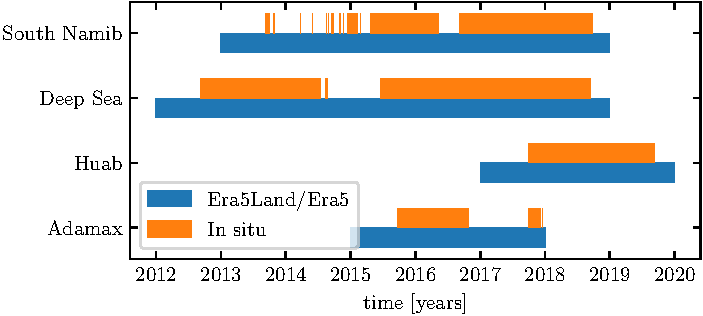
\includegraphics[scale=1]{Figures/Figure1_supp.pdf}
  \caption{Gant chart representing the usable time steps for the two data sets, for all stations.}
  \label{Fig1_supp}
\end{figure}

\begin{figure}
  \centering
  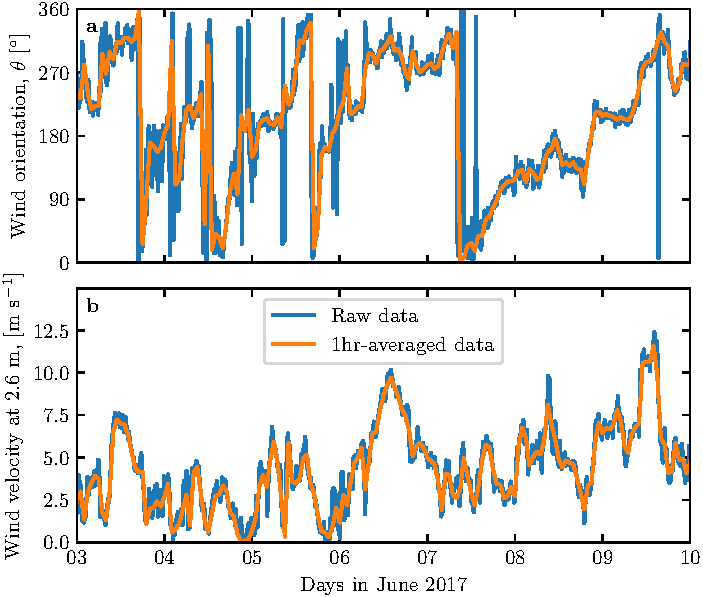
\includegraphics[scale=1]{Figures/Figure2_supp.pdf}
  \caption{Comparison between raw in situ wind measurements, and centered averaged data over one hour for the South Namib station. \textbf{a}: wind direction. \textbf{b}: wind velocity at the measurement height, 2.6 m.}
  \label{Fig2_supp}
\end{figure}

\section*{1. Shear velocity and calibration of the hydrodynamical roughness}
\label{calib_z0}

For each station, the hydrodynamic roughness is calibrated by finding the one that minimizes the relative difference $\delta$ between the wind vectors of both datasets:
\begin{equation}
  \label{metric_roughness}
      \delta = \frac{\sqrt{\langle\| \boldsymbol{u}_{*, \textrm{era}} - \boldsymbol{u}_{*, \textrm{station}} \|^{2}\rangle_{t}}}{\sqrt{ \langle \| \boldsymbol{u}_{*, \textrm{era}} \| \rangle_{t}\langle \| \boldsymbol{u}_{*, \textrm{station}} \| \rangle_{t}}}
\end{equation}



This $\delta$--parameter is computed for hydrodynamic roughness values ranging from $10^{-5}$~m to $10^{-2}$~m for the different stations. A shown by figure~\ref{Fig3_supp}, the minimum of $\delta$ in the space ($z_{0,\, \textup{Era}}$, $z_{0,\, \textup{in situ}}$) forms a line. We thus take the roughness of the Era5Land dataset as the typical value when sediment transport occurs, $10^{-3}$~m, corresponding to the thickness of the transport layer \citep{Sherman2007}. It leads for the Adamax, Deep Sea, Huab and South Namib stations values of $2.7~\textup{mm}$, $0.76~\textup{mm}$, $0.12~\textup{mm}$ and $0.48~\textup{mm}$, respectively.

The choice of the hydrodynamic roughness values only impacts the calculated shear velocities, but note the wind directions. As such, most of our conclusions are then independent of such a choice, and only the magnitude of the wind velocity attenuation in confined situation might be affected.


\begin{figure}
  \centering
  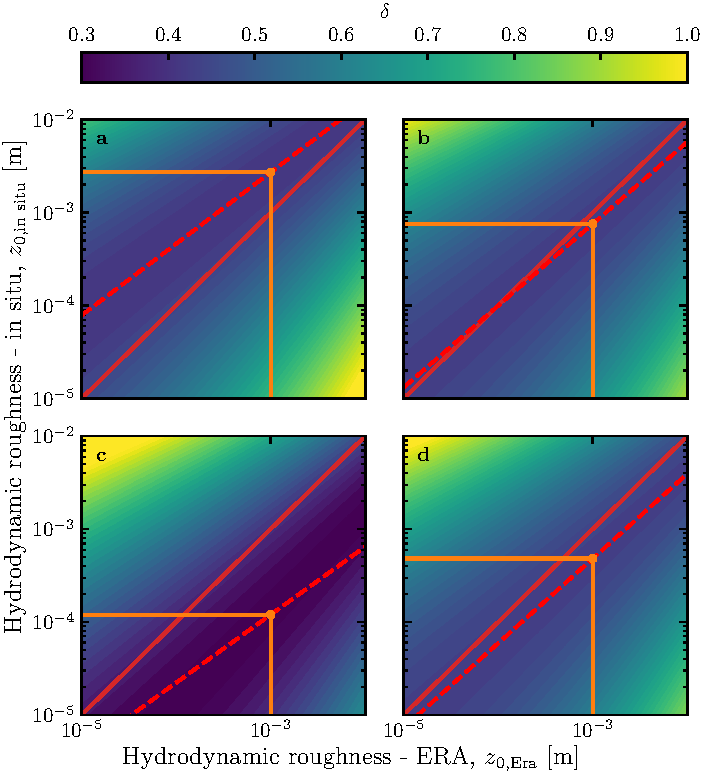
\includegraphics[scale=1]{Figures/Figure3_supp.pdf}
  \caption{Calibration of the hydrodynamic roughnesses. The metric $\delta$ defined in \eqref{metric_roughness} is represented in colorscale as a function of the hydrodynamic roughnesses chosen for the Era5-Land and in situ datasets, for the Adamax (\textbf{a}), Deep Sea (\textbf{b}), Huab (\textbf{c}) and South Namib (\textbf{d}) Stations. The red dashed and plain lines shows the minima of $\delta$ and the identity line. The orange lines and dots highlights the chosen the hydrodynamic roughnesses for the in situ datasets by imposing $z_{0, \textup{\textup{ERA}}} = 1~\textup{mm}$, leading for each station to $2.7~\textup{mm}$, $0.76~\textup{mm}$, $0.12~\textup{mm}$ and $0.48~\textup{mm}$, respectively.}
  \label{Fig3_supp}
\end{figure}


\begin{figure}
  \centering
  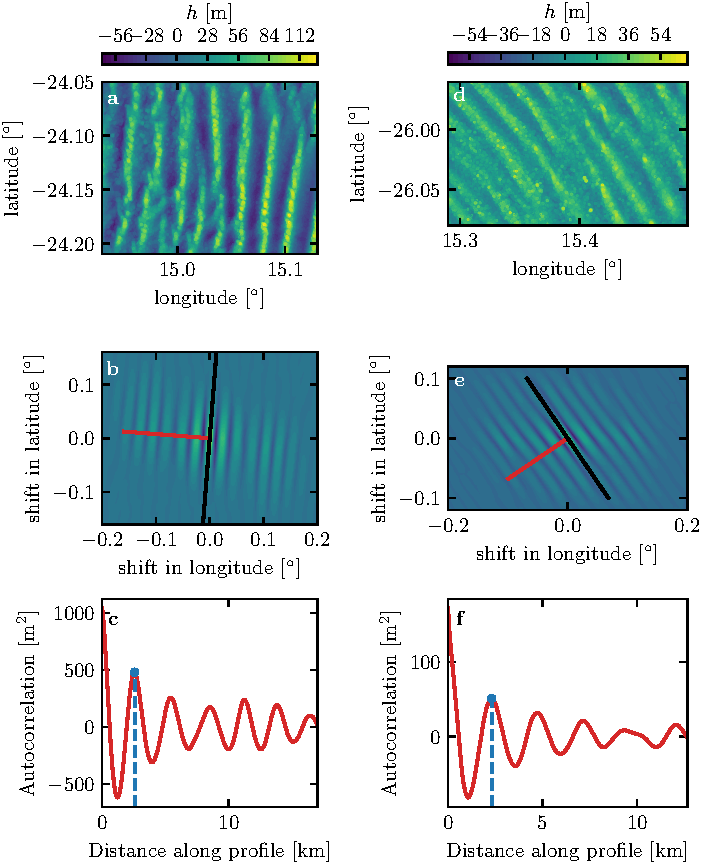
\includegraphics[scale=1]{Figures/Figure4_supp.pdf}
  \caption{Analysis of the DEMs of the Deep Sea (left column -- \textbf{a}, \textbf{b}, \textbf{c}) and South Namib (right column -- \textbf{d}, \textbf{e}, \textbf{f}) stations. \textbf{a--c}: Detrended topography (a second order polynomial is first fitted and then removed) . \textbf{b--d}: autocorrelation matrix shown in colorscale. The black line shows the detected orientation, and the red line the profile along which the wavelength is calculated, shown in \textbf{e--f}. The blue lines and dots show the first peak of the autocorrelation profile, whose horizontal position gives the characteristic wavelength of the dune pattern.}
  \label{Fig4_supp}
\end{figure}

\begin{figure}
  \centering
  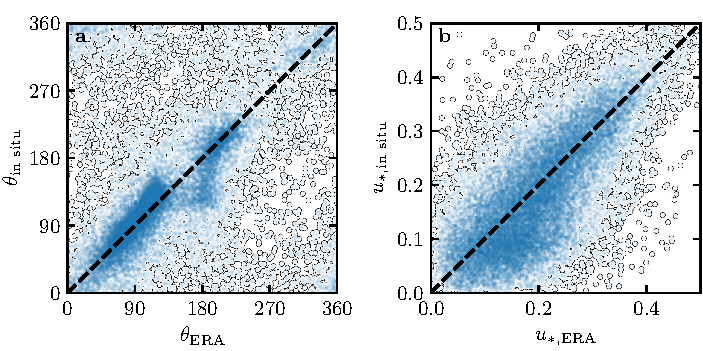
\includegraphics[scale=1]{Figures/Figure5_supp.pdf}
  \caption{Statistical agreement of the wind orientation (\textbf{a}) and velocity (\textbf{b}) between the Era5Land dataset and the in situ measurements for the Huab and Adamax stations. Note how the points are clustered around identity lines, black and dashed.}
  \label{Fig5_supp}
\end{figure}

\begin{figure}
  \centering
  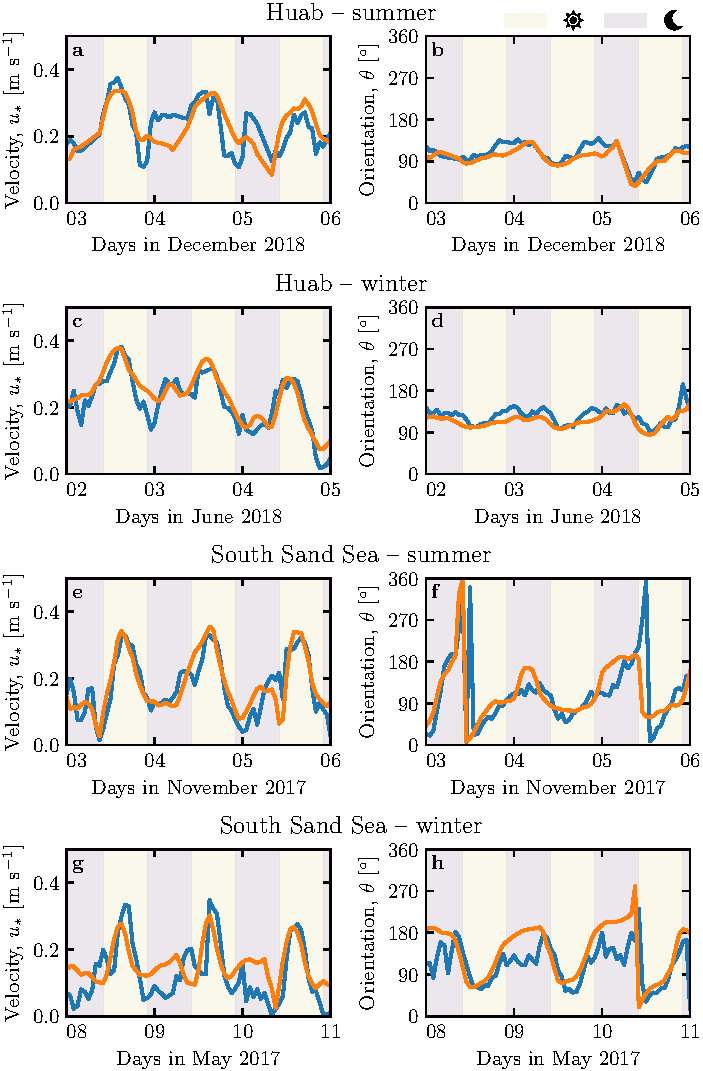
\includegraphics[scale=1]{Figures/Figure6_supp.pdf}
  \caption{Distributions of wind direction at the South Namib Station for the Era5Land climate reanalysis (orange) and the in situ measurements (blue). In each subplot, both distributions are plotted from the same time steps, selected with constraints on the wind direction (columns) and/or wind velocity (rows) in the Era5Land dataset. The grey dashed vertical lines indicate the dune orientation. The purple frame highlights the regime (small wind velocities, nocturnal summer wind) during which the wind data from both datasets differs. A similar figure can be obtained for the South Namib station (see Fig.~\ref{Fig3}).}
  \label{Fig6_supp}
\end{figure}

\begin{figure}
  \centering
  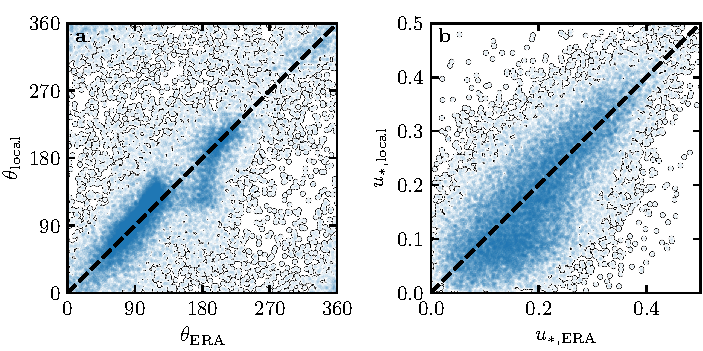
\includegraphics[scale=1]{Figures/Figure7_supp.pdf}
  \caption{Statistical comparison of the wind orientation between the Era5Land dataset and in situ measurements for the South Namib and Deep Sea stations, for different velocity ranges. \textbf{a}: $u_{*, \textup{\textup{ERA}}} < 0.1~\textup{m}~\textup{s}^{-1}$. \textbf{b}: $0.1 < u_{*, \textup{\textup{ERA}}} \leq 0.25~\textup{m}~\textup{s}^{-1}$. \textbf{c}: $u_{*, \textup{\textup{ERA}}} \geq 0.25~\textup{m}~\textup{s}^{-1}$. Note that the dune orientations measured are substracted to the wind orientation, which allows to plot both stations on the same graph. Black dashed lines indicates in situ orientations aligned with the dune crests (here $0^\circ$, $180^\circ$ and $360^\circ$ -- \textbf{a}, \textbf{b}), as well as the identity lines (\textbf{b}, \textbf{c}).}
  \label{Fig7_supp}
\end{figure}

\begin{figure}
  \centering
  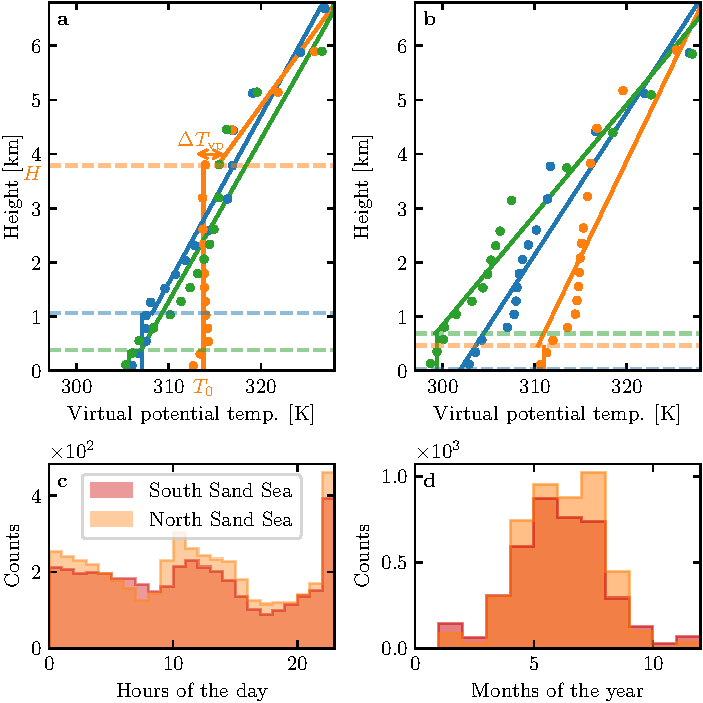
\includegraphics[scale=1]{Figures/Figure8_supp.pdf}
  \caption{Statistical comparison of the wind velocity between the Era5Land dataset and in situ measurements for the South Namib and Deep Sea stations. \textbf{a}: Nocturnal summer easterly wind. \textbf{b}: Diurnal southerly wind. Black dashed lines are identity lines. The angle ranges corresponding to diurnal and nocturnal summer winds are those taken in Fig.~\ref{Fig3} and Fig.~\ref{Fig6_supp}.}
  \label{Fig8_supp}
\end{figure}

\section*{2. Extraction of the ABL properties}

In order to estimate the relevant non-dimensional numbers, one need to estimate in addition to the wind and dune properties some parameters of the ABL. The Era5 dataset provides a direct bulk estimate of the ABL depth $H$ from a bulk Richardson number calculation, as well as vertical profiles of the geopotential $\phi$, temperature $T$ and specific humidity $e_{\textup{w}}$ at given pressure levels $P$. From these quantities, the virtual potential temperature, which takes into account the vertical pressure and humidity changes, can be calculated as:
\begin{equation}
  T_{\textup{vp}} = T\left(1 + \left[R_{\textup{M}} - 1\right]e_{\textup{w}}\right)\left(\frac{P_{0}}{P}\right)^{P_{\textup{c}}(1 - 0.24e_{\textup{w}})},
\end{equation}
where $P_{0} = 10^{5}~\textup{Pa}$ is the standard pressure, $P_{\textup{c}} = 0.2854$ the Poisson coefficient for dry air and $R_{\textup{M}}=1.61$ is the ratio between the melocular masses of dry air and water. The vertical coordinates are calculated as:
\begin{equation}
  z = \frac{\phi R_{\textup{t}}}{g R_{\textup{t}} - \phi},
\end{equation}
where $R_{\textup{t}} = 6356766~\textup{m}$ is the average Earth radius, and $g = 9.81~\textup{m}~\textup{s}^{-2}$ the gravitational acceleration.

Example of obtained vertical profiles of the virtual potential temperature are shown in Fig.~\ref{Fig9_supp}. On each of them, an average is computed below the ABL depth given by the Era5 dataset, and a linear function is fitted above.


Under the Boussinesq approximation, the temperature variations are assumed to induce most of those of the density, leading to $\Delta\rho/\rho \simeq \Delta T_{\textup{vp}}/T_{\textup{vp}}$. Here, $T_{\textup{vp}}/T_{\textup{vp}}$ is the relative virtual potential temperature jump at the capping, directly measured on the vertical profiles.

Following \citet{Tritton2012}, the relative density jump at the capping layer


\begin{figure}
  \centering
  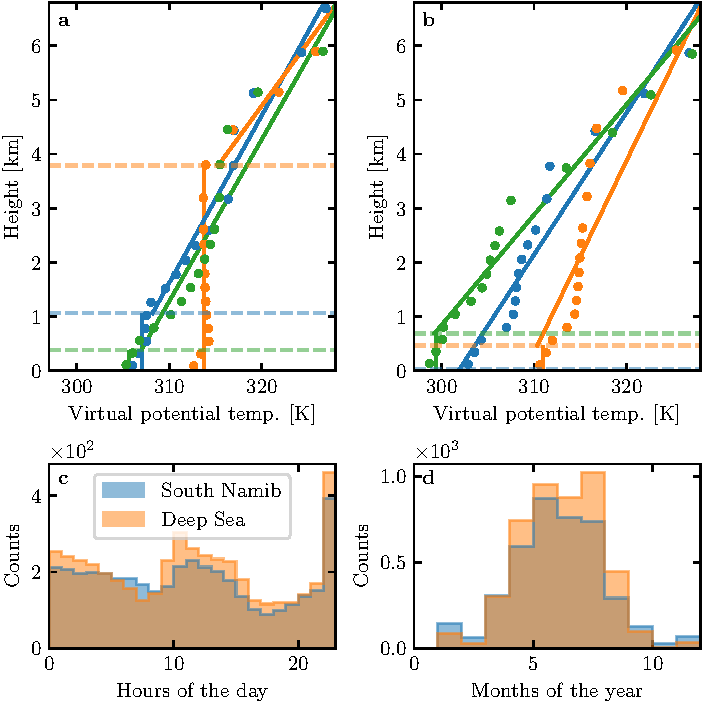
\includegraphics[scale=1]{Figures/Figure9_supp.pdf}
  \caption{\textbf{a}: Vertical profiles of the virtual potential temperature at 3 different time steps (blue - 29/11/2012 - 1100 UTC, orange - 21/03/2017 - 1200 UTC, green - 21/03/2017 - 2000 UTC) at the South Namib station. Dots: data from the ERA5 reanalysis. Transparent dashed lines: boundary layer height given by the ERA5 reanalysis, calculated from the bulk Richardson number \citep{seidel2012}. Plain lines: vertical (boundary layer) and linear (free atmosphere) fits to estimate the quantities in Fig.~\ref{Fig10_supp}. \textbf{b}: Examples of ill-processed vertical profiles at 3 different time steps (blue - 2/12/2013 - 2300 UTC, orange - 20/03/2017 - 0000 UTC, green - 14/07/2017 - 1400 UTC) at the South Namib station. \textbf{c}: Hourly distribution of ill-processed vertical profiles. \textbf{d}: Monthly distribution of ill-processed vertical profiles. \cg{These profiles are ill-processed because the temperature found at the boundary layer from the linear fit in the free-atm is smaller than the average one inside the boundary layer. This is an unstable situation, which does not allow to calculate the surface Froude number.}}
  \label{Fig9_supp}
\end{figure}

\begin{figure}
  \centering
  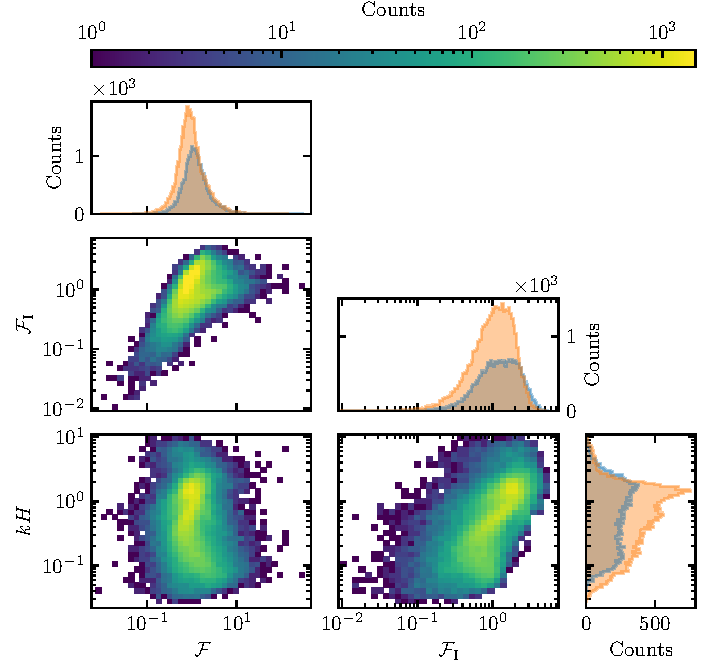
\includegraphics{Figures/Figure10_supp.pdf}
  \caption{Distributions of the meteorological parameters resulting from the processing of the Era5-Land data for the South Namib (blue) and the Deep Sea (orange) stations.}
  \label{Fig10_supp}
\end{figure}

\begin{figure}
  \centering
  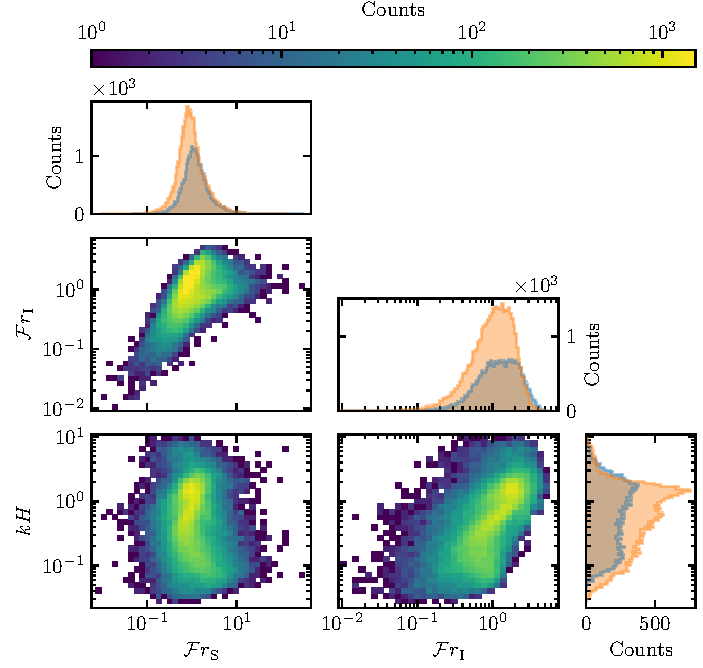
\includegraphics[scale=1]{Figures/Figure11_supp.pdf}
  \caption{Non-dimensional parameters distributions. For the marginal distributions, the orange correspond to the South Namib station, and the blue to the Deep Sea station.}
  \label{Fig11_supp}
\end{figure}

\begin{figure}
  \centering
  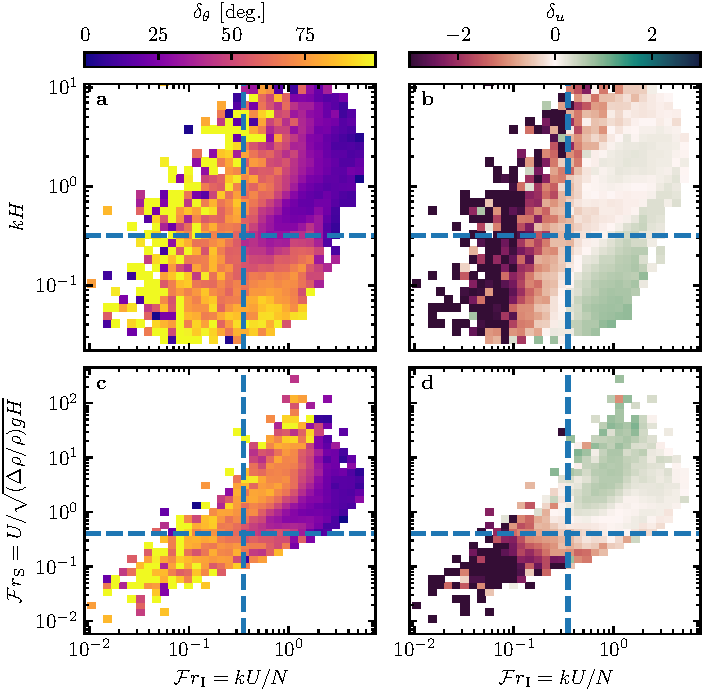
\includegraphics[scale=1]{Figures/Figure12_supp.pdf}
  \caption{Regime diagrams of the wind deviation $\delta_{\theta}$ and relative attenuation/amplification $\delta_{u}$ in the spaces $(\mathcal{F}r_{\textup{I}}, \, kH)$ and $(\mathcal{F}r_{\textup{I}}, \, \mathcal{F}r_{\textup{S}})$, containing the data from both the Deep Sea and South Namib stations. Blue dashed lines empirically delimit the different regimes. The point density in each bin of the diagrams is shown in Fig.~\ref{Fig11_supp}. The regime diagrams in the space $(\mathcal{F}r_{\textup{S}}, \, kH)$ are shown in Fig.~\ref{Fig5_supp}.}
  \label{Fig12_supp}
\end{figure}

\begin{figure}
  \centering
  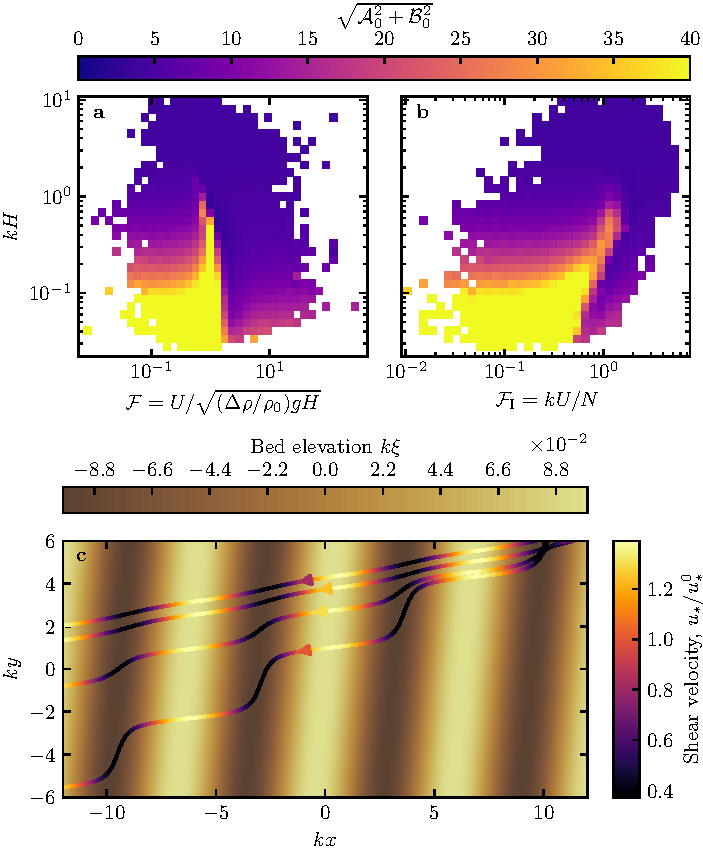
\includegraphics[scale=1]{Figures/Figure13_supp.pdf}
  \caption{Physical interpretation of the flow disturbance. (a) and (b) Magnitude of the disturbance induced by a sinusoidal topography calculated from the time series of the non-dimensional numbers presented in Figures~\ref{Fig4} and \ref{Fig5} using the linear model of \citet{andreotti2009}. (c) Shear velocity streamlines represented in the case of the Deep Sea station, for increasing values of $\sqrt{\mathcal{A}_{0}^{2} + \mathcal{B}_{0}^{2}}$. From the upper to the lower streamline, values of $\left(kH,\, Fr_{\textup{surface}},\, Fr_{\textup{internal}},\, \mathcal{A}_{0},\, \mathcal{B}_{0},\, \sqrt{\mathcal{A}_{0}^{2} + \mathcal{B}_{0}^{2}}\right)$ are (1.9, 0.6, 1.5, 3.4, 1.0, 3.5), (1.5, 0.3, 0.4, 4.8, 1.4, 5.0), (0.1, 3.5, 1.0, 8.6, 0.1, 8.6), (0.5, 0.05, 0.04, 9.6, 2.5, 9.9).}
  \label{Fig13_supp}
\end{figure}


\end{document}
